\documentclass[aspectratio=169]{beamer} % Format 16:9
\usepackage[utf8]{inputenc}
\usepackage{polski}
\usetheme[lang=pl,hr=true]{NewPwr}
\usepackage[T1]{fontenc}
\usepackage{graphicx}
\usepackage{hyperref}
\graphicspath{ {./img/} }

% DANE DO STRONY TYTUŁOWEJ
\title{Ucieczka z miasta}
\subtitle{Dlaczego na wsi żyje się lepiej niż w mieście?}
\author{Piotr Dryś}
\institute{Politechnika Wrocławska}
\date{\today}

\begin{document}
% SLAJD 1
{
\begin{frame}
    \titlepage
\end{frame}
}

% SLAJD 2
\begin{frame}{Zaliczenie zadania}
    \textbf{Link do repozytorium ze źródłami prezentacji:}
    
    \vspace{1cm}
    
    \begin{center}
        \url{https://github.com/Drysiu/Zadanie_LaTeX-beamer}
    \end{center}
    
    \vspace{1cm}
    \footnotesize
    Repozytorium zawiera pliki źródłowe (.tex, .bib, obrazki) bez plików pomocniczych.
\end{frame}

% SLAJD 3
\begin{frame}{Plan prezentacji}
    \tableofcontents
\end{frame}

    % SLAJD 4
\section{Streszczenie} 
\begin{frame}{Streszczenie i cel pracy}
    \begin{itemize}
        \item Tekst analizuje rosnący trend migracji z miast na wieś.
        \item Argumentuje się, że życie poza aglomeracją oferuje wyższą jakość codziennego funkcjonowania.
        \item Wskazane są cztery najważniejsze obszary przewagi wsi: 
        \begin{itemize}
            \item zdrowie,
            \item relacje społeczne,
            \item ekonomia,
            \item psychologia.
        \end{itemize}
        \item \textbf{Wniosek:} Ucieczka z miasta jest świadomym wyborem na rzecz odzyskania równowagi życiowej i polepszenia psychiki.
    \end{itemize}
\end{frame}

% SLAJD 5
\section{Wprowadzenie}
\begin{frame}{Miasto a wieś - obecne trendy}
    \begin{itemize}
        \item Miasto jest z natury bardziej atrakcyjne (bliskość pracy, edukacji, rozrywki).
        \item Wsie i mniejsze miejscowości zyskują jednak coraz więcej mieszkańców.
        \item Główny czynnik zmiany: możliwość pracy zdalnej.
    \end{itemize}
\end{frame}

% SLAJD 6
\begin{frame}{Przyczyny migracji}
    \begin{itemize}
        \item Wzrastające ceny mieszkań w miastach.
        \item Ucieczka od miejskiego hałasu.
        \item Chęć życia w spokoju i ciszy.
        \item Zniechęcające cechy miasta: ciągła pogoń, stanie w korkach, wysokie koszty życia.
    \end{itemize}
\end{frame}

% SLAJD 7
\begin{frame}{Wizualizacja}
    \begin{figure}
        \centering
        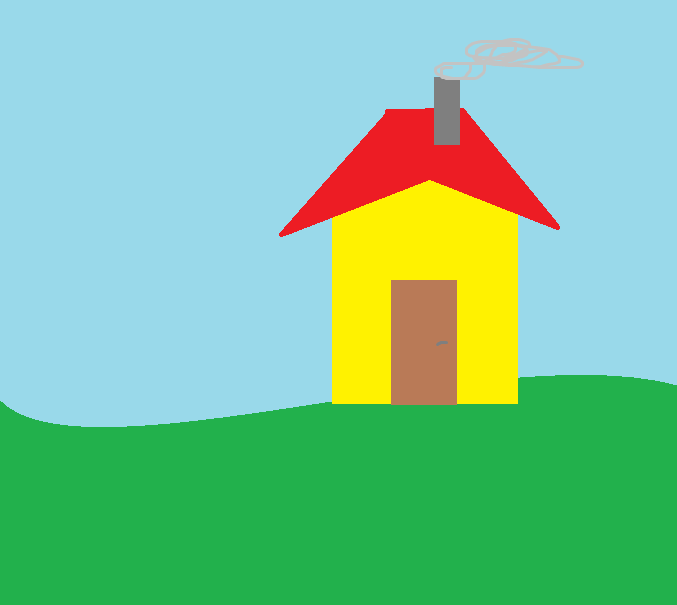
\includegraphics[height=0.7\textheight]{wies.png} 
        \caption{Sielski krajobraz wiejski}
    \end{figure}
\end{frame}

% SLAJD 8
\begin{frame}{Kontakt z naturą i zdrowie}
    \begin{itemize}
        \item Na wsi występuje znacznie bliższy kontakt z naturą (lasy, pola zamiast betonu).
        \item Czyste powietrze zamiast spalin.
        \item Korzyści zdrowotne:
        \begin{itemize}
            \item mniej alergii,
            \item niższy poziom stresu.
        \end{itemize}
        \item Naturalna motywacja do aktywności (spacery, rower) bez konieczności szukania zatłoczonego parku.
    \end{itemize}
\end{frame}

% SLAJD 9
\begin{frame}{Relacje społeczne}
    \begin{itemize}
        \item \textbf{Miasto:} Mimo tłumów, łatwo o anonimowość i samotność.
        \item \textbf{Wieś:} Społeczności są mniejsze i bardziej zżyte.
        \item Sąsiedzi się znają i pomagają sobie.
        \item Tworzenie poczucia wspólnoty daje większe bezpieczeństwo i oparcie w trudnych chwilach.
    \end{itemize}
\end{frame}

% SLAJD 10
\begin{frame}{Przestrzeń życiowa}
    \begin{itemize}
        \item Porównanie ekonomiczne: Małe mieszkanie z widokiem na blok (miasto) vs Dom z własnym ogrodem (wieś).
        \item Nowa jakość życia na wsi:
        \begin{itemize}
            \item miejsce na grilla,
            \item przestrzeń do zabawy dla dzieci,
            \item możliwość wypicia kawy na własnym tarasie w otoczeniu zieleni (brak miejskiego zgiełku).
        \end{itemize}
    \end{itemize}
\end{frame}
    \section{Aspekty zdrowotne i środowiskowe}

% SLAJD 11
\begin{frame}{Jakość środowiska naturalnego}
    \begin{itemize}
        \item \textbf{Fundament zdrowia:} Bezpośredni kontakt z nieskażoną przyrodą.
        \item \textbf{Czyste powietrze i cisza:} 
        \begin{itemize}
            \item Redukcja ryzyka chorób cywilizacyjnych (alergie, astma).
            \item Brak permanentnego hałasu miejskiego.
        \end{itemize}
        \item \textbf{Psychika:} Wszechobecna zieleń sprzyja regeneracji psychicznej, redukcji stresu i odnalezieniu wewnętrznej harmonii.
    \end{itemize}
\end{frame}

% SLAJD 12
\begin{frame}{Analiza zanieczyszczeń (PM2.5)}
    \begin{table}
        \centering
        \small
        \caption{Porównanie średniorocznego stężenia pyłu PM2.5 \cite{link1}}
        \begin{tabular}{|l|c|c|}
            \hline
            \textbf{Lokalizacja} & \textbf{Stężenie ($\mu$g/m$^3$)} & \textbf{Norma WHO} \\ \hline
            Duże miasto (Kraków) & 25-35 & 5 \\ \hline
            Wieś (brak przemysłu) & 10-15 & 5 \\ \hline
        \end{tabular}
    \end{table}

    \vspace{0.5cm}
    
    Na wsi stężenie szkodliwego pyłu jest nawet \textbf{2-3 razy niższe}.
    
    \begin{block}{Wzór na stężenie masowe pyłu}
        $$ \text{C}_{\text{PM}_{2.5}} = \frac{m_{\text{PM}_{2.5}}}{V} $$
    \end{block}
\end{frame}

\section{Aspekty społeczne i ekonomiczne}

% SLAJD 13
\begin{frame}{Społeczność i tożsamość}
    \begin{columns}
        \begin{column}{0.5\textwidth}
            \textbf{Więzi społeczne:}
            \begin{itemize}
                \item Brak miejskiej anonimowości.
                \item Relacje oparte na zaufaniu i pomocy sąsiedzkiej (kapitał społeczny).
                \item Wyższe poczucie bezpieczeństwa i oparcia w grupie.
            \end{itemize}
        \end{column}
        
        \begin{column}{0.5\textwidth}
            \textbf{Kultura i tradycja:}
            \begin{itemize}
                \item Żywy kontakt z lokalnym folklorem i obrzędami.
                \item Ochrona przed globalizacją kulturową.
                \item Wzmacnianie tożsamości regionalnej i międzypokoleniowej.
            \end{itemize}
        \end{column}
    \end{columns}
\end{frame}

% SLAJD 14
\begin{frame}{Przestrzeń, wolność i ekonomia}
    \begin{itemize}
        \item \textbf{Ekonomia:} Niższe ceny nieruchomości pozwalają na posiadanie domu z ogrodem (zamiast ciasnego mieszkania).
        \item \textbf{Wolność osobista:} 
        \begin{itemize}
            \item Większa prywatność i brak tłumów.
            \item Możliwość realizacji głośnych hobby czy hodowli zwierząt.
        \end{itemize}
        \item \textbf{Niezależność:} Możliwość częściowej samowystarczalności (własne uprawy) i niezależności finansowej.
    \end{itemize}
\end{frame}

% SLAJD 15
\begin{frame}{Rytm życia i rozwój umiejętności}
    \begin{itemize}
        \item \textbf{Slow Life:} Ucieczka od pośpiechu i presji czasu na rzecz życia zgodnego z rytmem natury.
        \item \textbf{Wartości:} Odchodzenie od konsumpcjonizmu na rzecz autentycznych potrzeb i relacji.
        \item \textbf{Praktyczne umiejętności:}
        \begin{itemize}
            \item Rozwój zaradności (prace w ogrodzie, naprawy).
            \item Poczucie sprawczości, które zanika w miejskim stylu życia.
            \item Szacunek dla zasobów i pracy fizycznej.
        \end{itemize}
    \end{itemize}
\end{frame}
    \section{Miasto a wieś - analiza porównawcza}

% SLAJD 16
\begin{frame}{Wyzwania życia w mieście \cite{link2}}
    \begin{itemize}
        \item \textbf{Stres i presja czasu:}
        \begin{itemize}
            \item Miasto to nieustanny wyścig z terminami i ludźmi.
            \item Nadmiar bodźców generuje chroniczny stres.
            \item \textit{Wieś:} Spokojniejszy rytm pozwala na regenerację.
        \end{itemize}
        
        \item \textbf{Koszty życia:}
        \begin{itemize}
            \item Astronomiczne ceny mieszkań ("mała przestrzeń za fortunę").
            \item \textit{Wieś:} Ten sam budżet pozwala na dom z ogrodem.
        \end{itemize}

        \item \textbf{Wszechobecny hałas:}
        \begin{itemize}
            \item Syreny, ruch uliczny, brak ciszy nocnej (pogorszony sen).
            \item \textit{Wieś:} Cisza przerywana jedynie odgłosami natury.
        \end{itemize}
    \end{itemize}
\end{frame}

% SLAJD 17
\begin{frame}{Otoczenie społeczne i przyrodnicze}
    \begin{itemize}
        \item \textbf{Deficyt natury:} Miasto to "betonowa dżungla". Brak codziennego dostępu do zieleni negatywnie wpływa na samopoczucie.
        
        \item \textbf{Przestrzeń i prywatność:}
        \begin{itemize}
            \item W bloku słychać sąsiadów przez ścianę.
            \item Wieś oferuje własne podwórko i brak tłoku.
        \end{itemize}

        \item \textbf{Relacje międzyludzkie:}
        \begin{itemize}
            \item \textit{Miasto:} Anonimowość i samotność w tłumie.
            \item \textit{Wieś:} Silne więzi sąsiedzkie i wzajemna pomoc.
        \end{itemize}

        \item \textbf{Bezpieczeństwo:} Niższy wskaźnik przestępczości na wsi i brak anonimowości sprzyjają bezpieczeństwu (szczególnie dzieci).
    \end{itemize}
\end{frame}

% SLAJD 18
\section{Tempo życia}
\begin{frame}{Różnice w codziennym tempie życia}
    \begin{columns}
        \begin{column}{0.5\textwidth}
            \textbf{\textcolor{red}{Miasto (Dyktando zegarka)}}
            \begin{itemize}
                \item Dzień precyzyjnie zaplanowany ("wypełniony po brzegi").
                \item Dominacja pośpiechu, korków i multitaskingu.
                \item Posiłki w biegu (lunch przy biurku).
                \item Wieczorem: szukanie kolejnych bodźców zamiast wyciszenia.
            \end{itemize}
        \end{column}

        \begin{column}{0.5\textwidth}
            \textbf{\textcolor{green!60!black}{Wieś (Cykl natury)}}
            \begin{itemize}
                \item Tempo wyznaczają pory roku i dnia, a nie kalendarz.
                \item Spokojniejsze poranki bez presji bycia "wszędzie naraz".
                \item Praca przeplatana odpoczynkiem (np. w ogrodzie).
                \item Wieczory spędzane z bliskimi na wyciszeniu.
            \end{itemize}
        \end{column}
    \end{columns}
\end{frame}
    \section{Poczucie szczęścia a miejsce zamieszkania}

% SLAJD 19
\begin{frame}{Wpływ otoczenia na psychikę}
    \begin{itemize}
        \item \textbf{Wybór egzystencjalny:} Decyzja o miejscu zamieszkania to nie tylko logistyka, ale czynnik kształtujący codzienność i relacje.
        \item \textbf{Miasto (Przeciążenie):}
        \begin{itemize}
            \item Permanentne przebodźcowanie (hałas, światła, reklamy).
            \item "Wyścig szczurów" prowadzi do chronicznego stresu i wypalenia.
        \end{itemize}
        \item \textbf{Wieś (Mindfulness):}
        \begin{itemize}
            \item Rytm podyktowany naturą pozwala na regenerację.
            \item \textit{Attention Restoration Theory:} Kontakt z przyrodą odnawia zasoby uwagi i zwiększa kreatywność.
        \end{itemize}
    \end{itemize}
\end{frame}

% SLAJD 20
\begin{frame}{Relacje społeczne i ekonomia}
    \begin{columns}
        \begin{column}{0.5\textwidth}
            \textbf{Paradoks miasta:}
            \begin{itemize}
                \item Tłum ludzi, a jednak samotność.
                \item Relacje transakcyjne i powierzchowne.
                \item Brak poczucia przynależności.
            \end{itemize}
            
            \vspace{0.3cm}
            \textbf{Siła wsi:}
            \begin{itemize}
                \item Model wspólnotowy i kapitał społeczny.
                \item Poczucie bezpieczeństwa dzięki pomocy sąsiedzkiej.
            \end{itemize}
        \end{column}

        \begin{column}{0.5\textwidth}
            \textbf{Aspekt ekonomiczny i zdrowotny:}
            \begin{itemize}
                \item Miasto: Wyższe zarobki, ale ogromne koszty życia (presja finansowa).
                \item Zdrowie: Smog \cite{link3} i hałas vs czyste powietrze.
                \item Wieś: Ten sam budżet = wyższy standard (dom, ogród, pasje).
            \end{itemize}
        \end{column}
    \end{columns}
\end{frame}

% SLAJD 21
\begin{frame}{Zestawienie czynników szczęścia \cite{link2, link3}}
    \begin{table}
        \centering
        \tiny
        \caption{Porównanie wpływu środowiska na dobrostan}
        \begin{tabular}{|l|p{3.5cm}|p{3.5cm}|}
            \hline
            \textbf{Czynnik} & \textbf{Miasto} & \textbf{Wieś / Przedmieścia} \\ \hline
            Poziom stresu & Wysoki, chroniczny (pośpiech, hałas) & Niski, epizodyczny (spokój) \\ \hline
            Więzi społeczne & Anonimowość, powierzchowność & Wspólnota, głębokie relacje \\ \hline
            Środowisko & Smog, hałas & Czyste powietrze, cisza \\ \hline
            Natura & Ograniczona (parki) & Nieograniczona (lasy, pola) \\ \hline
            Finanse & Wysoka presja (drogie życie) & Niższe koszty, wyższy standard \\ \hline
            Bezpieczeństwo & Niższe (anonimowość) & Wyższe (znajomość sąsiadów) \\ \hline
            Tempo życia & Narzucone, szybkie & Zgodne z naturą, wolne \\ \hline
        \end{tabular}
    \end{table}
    
    \vspace{0.2cm}
    \scriptsize
    \textbf{Wniosek:} Obszary wiejskie zapewniają solidniejsze fundamenty dla zdrowia psychicznego i bezpieczeństwa.
\end{frame}

% SLAJD 22
\begin{frame}{Podsumowanie: Świadomy wybór}
    \begin{block}{Definicja szczęścia}
        Szczęście nie zależy od liczby kin czy restauracji, ale od jakości snu, głębokości relacji i poczucia kontroli nad życiem.
    \end{block}

    \begin{itemize}
        \item Migracja na wieś (wspierana pracą zdalną) to świadome odrzucenie ciągłej pogoni za wzrostem.
        \item Wybór równowagi, spokoju i autentyczności.
        \item W kluczowych obszarach dobrostanu, wieś oferuje więcej niż metropolia.
    \end{itemize}
\end{frame}
    \section{Aspekty ekonomiczne}

% SLAJD 23
\begin{frame}{Nieruchomości – przepaść w cenie \cite{link4}}
    Wstęp: Mimo wyższych zarobków w mieście, realna jakość życia za te same pieniądze jest niższa.

    \vspace{0.5cm}

    \begin{columns}
        \begin{column}{0.48\textwidth}
            \textbf{\textcolor{red}{W mieście:}}
            \begin{itemize}
                \item Ogromna kwota za mały metraż.
                \item Przestrzeń ograniczona do mieszkania w bloku.
                \item Widok: często ściana sąsiedniego budynku.
            \end{itemize}
        \end{column}
        
        \begin{column}{0.48\textwidth}
            \textbf{\textcolor{green!60!black}{Na wsi:}}
            \begin{itemize}
                \item Cena mieszkania = Przestronny dom.
                \item Własny ogród i prywatność.
                \item Nieporównywalnie lepsze warunki dla rodziny.
            \end{itemize}
        \end{column}
    \end{columns}
\end{frame}

% SLAJD 24
\begin{frame}{Codzienne wydatki i styl życia \cite{link5}}
    \begin{columns}
        \begin{column}{0.48\textwidth}
            \textbf{\textcolor{red}{Koszty miejskie:}}
            \begin{itemize}
                \item Droższe usługi i parkingi.
                \item Wyższe ceny podstawowych zakupów.
                \item Pokusy drogich rozrywek.
                \item Środowisko sprzyjające konsumpcjonizmowi (obciążenie portfela).
            \end{itemize}
        \end{column}
        
        \begin{column}{0.48\textwidth}
            \textbf{\textcolor{green!60!black}{Oszczędności wiejskie:}}
            \begin{itemize}
                \item Dostęp do tańszej, lokalnej żywności.
                \item Niższe koszty usług.
                \item Darmowa rekreacja na łonie natury.
                \item Życie bez ciągłej presji finansowej.
            \end{itemize}
        \end{column}
    \end{columns}
\end{frame}

% SLAJD 25
\begin{frame}{Podsumowanie finansowe \cite{link5}}
    \begin{table}
        \centering
        \small
        \caption{Bilans zysków i strat}
        \begin{tabular}{|l|l|l|}
            \hline
            \textbf{Kategoria} & \textbf{Miasto} & \textbf{Wieś} \\ \hline
            Mieszkanie & Bardzo drogo, ciasno & Umiarkowanie, przestronnie \\ \hline
            Wydatki & Wysokie (pokusy) & Niskie (lokalne produkty) \\ \hline
            Jakość za cenę & Niska & Wysoka \\ \hline
        \end{tabular}
    \end{table}

    \vspace{0.5cm}

    \begin{block}{Wniosek: Siła nabywcza}
        Na wsi za każdą zarobioną złotówkę można kupić znacznie więcej przestrzeni, spokoju i lepszej jakości życia.
    \end{block}
\end{frame}

% SLAJD 26
\section{Podsumowanie}
\begin{frame}{Podsumowanie: Dwie filozofie życia}
    \begin{itemize}
        \item Wybór "Miasto vs Wieś" to starcie dwóch różnych filozofii życiowych.
        \item Miasto, mimo pozornej atrakcyjności, przegrywa w kluczowych kategoriach ludzkich potrzeb.
        \item Ucieczka z metropolii to nie kaprys, lecz \textbf{świadome poszukiwanie równowagi} w świecie zdominowanym przez pośpiech.
        \item Wieś daje szansę na odzyskanie kontroli nad czasem i budowanie autentycznych relacji.
    \end{itemize}

    \vspace{0.3cm}

    \begin{alertblock}{Nowa definicja sukcesu}
        Z dala od zgiełku sukcesu nie mierzy się pieniędzmi, lecz prawdziwą jakością życia, spokojem ducha i poczuciem przynależności.
    \end{alertblock}
\end{frame}
    \section*{Zakończenie}

% SLAJD 27
\begin{frame}
    \centering
    \vspace*{\fill}
    
    {\Huge \textbf{Dziękuję za uwagę!}}
    
    \vspace*{\fill}
\end{frame}
    \section{Literatura}

% SLAJD 28
\begin{frame}[allowframebreaks]
    \frametitle{Bibliografia}
    
    \footnotesize 

    \begin{thebibliography}{9}

        \bibitem{link1}
        \emph{Powietrze w Polsce – ranking najbardziej i najmniej zanieczyszczonych miast}, Polska w Praktyce, \url{https://polskawpraktyce.pl/powietrze-w-polsce-ranking-najbardziej-i-najmniej-zanieczyszczonych-miast.html} [dostęp: 11.01.2026].

        \bibitem{link2}
        \emph{Jakość życia}, Główny Urząd Statystyczny, \url{https://stat.gov.pl/obszary-tematyczne/warunki-zycia/jakosc-zycia/} [dostęp: 11.01.2026].

        \bibitem{link3}
        \emph{Portal Jakość Powietrza}, Główny Inspektorat Ochrony Środowiska, \url{https://powietrze.gios.gov.pl/pjp/home} [dostęp: 11.01.2026].

        \bibitem{link4}
        Polski Instytut Ekonomiczny, \url{https://pie.net.pl/} [dostęp: 11.01.2026].

        \bibitem{link5}
        Obserwator Finansowy, \url{https://www.obserwatorfinansowy.pl/} [dostęp: 11.01.2026].

    \end{thebibliography}
\end{frame}
    
\end{document}